\documentclass[3p,12pt,authoryear]{elsarticle}

\usepackage[colorlinks=true,citecolor=blue,linkcolor=blue]{hyperref}
\usepackage{amsmath,amssymb}
\usepackage{epsfig}  
\usepackage{graphicx}               % Standard graphics package  
\usepackage{url}
\usepackage{hyperref}
\usepackage{color}
\usepackage{listings}

\usepackage{chngcntr}
\counterwithin{figure}{section}

\newcommand{\bra}[1]{\ensuremath{\left\langle#1\right|}}
\newcommand{\ket}[1]{\ensuremath{\left|#1\right\rangle}}
\newcommand{\bracket}[2]{\ensuremath{\left\langle#1 \vphantom{#2}\right| \left. #2 \vphantom{#1}\right\rangle}}
\newcommand{\matrixel}[3]{\ensuremath{\left\langle #1 \vphantom{#2#3} \right| #2 \left| #3 \vphantom{#1#2} \right\rangle}}
\newcommand{\bls}{\begin{lstlisting}}
\newcommand{\els}{\end{lstlisting}}

\newcommand{\ttf}{\ttfamily}

\newcommand{\pa}[2]{\frac{\partial #1}{\partial #2}}
\newcommand{\p}[1]{\partial_{#1}}

\definecolor{mauve}{rgb}{1,0,1}
\definecolor{dkgreen}{rgb}{0,0.6,0}
% \definecolor{gray}{rgb}{0.5,0.5,0.5}
% \definecolor{mauve}{rgb}{0.58,0,0.82}

\lstset{language=C++,
%   aboveskip=3mm,
%   belowskip=3mm,
%   showstringspaces=false,
%   columns=flexible,
   basicstyle={\small\ttfamily},
%   numbers=none,
%   numberstyle=\tiny\color{gray},
   morekeywords={SU\_vector,string,Body,Track,array1D,array2D,array3D},   
   keywordstyle=\color{blue},
   deletekeywords={const},
   keywords=[2]{const},
   keywordstyle={[2]\ttfamily\color{red}},
   deletekeywords={operator},
   keywords=[3]{operator},
   keywordstyle={[3]\ttfamily\color{dkgreen}},
   commentstyle=\color{dkgreen},
   stringstyle=\color{mauve},
%   breaklines=true,
%   breakatwhitespace=true
%   tabsize=3
}

\begin{document}

\begin{frontmatter}

\title{$\nu$-SQuIDS: A toolbox for neutrino oscillation experiments.\tnoteref{t1}}

\author[uw,wipac]{Carlos Alberto Arg\"uelles Delgado}
\ead{arguelles@wisc.edu}
\author[uw,wipac]{Jordi Salvado Serrat}
\ead{salvadoserra@wisc.edu}
\address[uw]{Department of Physics, University of Wisconsin, Madison, WI 53706, USA} 
\address[wipac]{Wisconsin IceCube Particle Astrophysics Center, Madison, WI 53703, USA}

\tnotetext[t1]{The code can be found in \url{http://icecube.wisc.edu/\~carguelles/nusquids}}

\journal{Computer Physics Communications}

\begin{abstract}
The Neutrino Simple Quantum Integro-Differential equation Solver ($\nu$-SQuIDS) is a C++ code based on SQuIDS that propagates an ensemble of neutrinos through a given media, e.g. Sun, Earth, Vacuum, etc, while considering, in a consistent way, the effect of neutrino oscillations, with coherent matter interactions, and non coherent interactions. The code has been design to be accurate and flexible, while at the same time maintain excellent performance. Furthermore, the user can easily change the neutrino oscillation parameters, propagation medium, and easily incorporate new oscillation physics. 
\end{abstract}

\begin{keyword}
Neutrino oscillation, phenomenology, collective neutrino behavior, numerical techniques
\end{keyword}

\end{frontmatter}

\hypersetup{linkcolor=black}
\tableofcontents
\hypersetup{linkcolor=blue}

\section{Introduction}
\label{sec:intro} 

During the last decades a plethora of evidence that neutrinos change flavor as they propagate macroscopical distances due to the nonalignment of their mass and flavor eigenstates has accumulated from solar, atmospheric, accelerator, and reactor experiments \citep{Mohapatra:qv,Gouvea:2013fj}. Thanks to these remarkable experimental results and related theoretical calculations the {\it neutrino-mass induced flavor oscillation paradigm} \citep{fukugita2003physics,Akhmedov:1999uz,Balantekin:2013kc} has been firmly established and the three mixing angles, that parametrize the lepton mixing matrix, together with the two square mass differences have been measured to good precision \citep{gonzalez2012global}. Furthermore, it is the task of on going and future experiments to determine the neutrino mass ordering and the Dirac CP-violating phase \citep{Agarwalla:2012mz}.

Even though most of the data can be explained in the standard three neutrino framework some {\it puzzling} anomalies still remain \citep{LSND,Mention:2011rr,MiniBoone:2012dn}. These may be explained by introducing new {\it neutrino} states, often refer to as {\it light sterile neutrinos} \citep{kopp2013sterile,Conrad:2013oq,Abazajian:2012rf}. Moreover, other new physics scenarios such as the possibility of non standard interactions \citep{Kopp:2014nosterile,Pospelov:2011dp} have also been considered. Also the interplay between cosmology and neutrino oscillation has been widely studied in the literature as well as a playground for new physics scenarios \citep{Archidiacono:2014oq,Dasgupta:2013la,Saviano:2014bs}. In general, neutrino physics constitutes an excellent prove for fundamental physics \citep{Hewett:2012et}.

It is clear that a tool is needed to correctly solve the neutrino propagation problem, i.e. vacuum oscillation and matter induced interactions \citep{Blennow:2013hi}. In particular, when only neutrino oscillations are important  softwares such as {\ttf GLoBES} \citep{Huber:2007ji} or {\ttf nuCRAFT} \citep{Wallraff:2014vl} have been made public. Unfortunately, when non coherent interactions are important they are no longer applicable. Furthermore, the ability to allow the user to incorporate new physics models and/or change the propagation medium is also limited. {\ttf nuSQuIDS} pretends to address all of these problems by providing a highly customizable package while at the same time remain numerically efficient.

The rest of the paper is organized as follows: in section \ref{sec:theory} we review neutrino oscillation theory and establish notation; in section \ref{sec:code} we describe the code; in section \ref{sec:examples} we exemplify the code and test it in benchmark scenarios. Finally, section \ref{sec:conclu} presents concluding remarks.

\section{Theory}
\label{sec:theory} 
\let\thefootnote\relax\footnotetext{We set $c = \hbar = 1$.} 

We can represent the neutrino state using the density matrix formalism, e.g. in the weak-interaction flavor eigenstate basis $\{\ket{\nu_\alpha}\}$  it can be written as

\begin{equation}
\rho = \sum_\alpha \phi_\alpha \ket{\nu_\alpha}\bra{\nu_\alpha} 
\label{eq:state}
\end{equation}

where $\phi_\alpha$ specifies the flavor content. Another important representation are the mass eigenstates $\{ \ket{\nu_i}  \}$, which are related to the former by

\begin{equation}
\ket{\nu_\alpha} = \sum_i U_{\alpha i} \ket{\nu_i} 
\label{eq:changebasis}
\end{equation}

where $U$ is the unitary lepton mixing matrix. It is customary to parametrize the mixing matrix $U$ with mixing angles, $\{\theta_{ij}\}$, and CP phases, $\{ \delta_{ij} \}$; for example when considering the standard 3 flavor paradigm the following parametrization is often used

\begin{equation}
U
=
\begin{pmatrix}
c_{12} c_{13} & s_{12} c_{13} & s_{13} e^{-i\delta_{13}} \\ 
- s_{12} c_{23} - c_{12} s_{23} s_{13} e^{i\delta_{13}} & c_{12} c_{23} - s_{12} s_{23} s_{13} e^{i\delta_{13}} & s_{23} c_{13} \\
s_{12}s_{23} -c_{12}c_{23}s_{13}e^{i\delta_{13}} & - c_{12} s_{23} - s_{12} c_{23} s_{13} e^{i\delta_{13}} & c_{23} c_{13}
\end{pmatrix}
\,,
\label{eq:U}
\end{equation}

where $c_{ij} = \cos \theta_{ij}$, $s_{ij} = \sin \theta_{ij}$. In the 3 flavor scenario we use the aforementioned parametrization (with values from \citep{gonzalez2012global}) and when more flavors are considered we used the prescription given in \citet{SQUIDS}. Furthermore, the neutrino ensemble evolution is described by the following Liouville equation

\begin{equation}
\pa{\rho(E)}{x} = -i [ H (E,x), \rho(E) ]~.
\label{eq:schrodinger}
\end{equation}

In general we can always split the Hamiltonian, $H$, into a time dependent and independent parts. In particular, for neutrino oscillations the following splitting is convenient

\begin{subequations}
\label{eq:hamiltonian}
\begin{align}
H(E,x) &= H_0(E)  + H_{1}(E,x) \\
H_0 (E) &= \frac{1}{2E} {\rm diag}( 0 , \Delta m^2_{21},\Delta m^2_{31},...,\Delta m^2_{i1},...,\Delta m^2_{n1}) \label{eq:h0} \\
H_1 (E,x) &= \sqrt{2} G_F U^\dagger {\rm diag} ( N_e(x) - N_n(x)/2, -N_n(x)/2, -N_n(x)/2 , 0,...,0 )U\label{eq:hi} 
\end{align}
\end{subequations}

where $n$ is the number of neutrino flavors, $G_F$ is the Fermi constant, $\Delta m^2_{i1}$ are the neutrino mass splittings, and, finally, $N_e(x)$ and $N_n(x)$ are the electron and nucleon number densities along the neutrino path. On writing these equations we have used the convention that the first three flavor eigenstates corresponds to $\nu_e$, $\nu_\mu$, and $\nu_\tau$, while the rest are assume to be sterile neutrinos. Furthermore, $H_0$ arrises from the neutrino kinetic term, where as $H_1$ incorporates the matter potential, i.e. coherent forward scattering interactions \citep{Mikheev:1986gs,Mikheev:1986wj,Wolfenstein:1977ue}. Given this splitting it is convenient to change to the so called {\it interaction picture} , generated by $H_0$, defined by the following transformation for a given operator $O$

\begin{equation}
O \to \bar{O}(x)=exp(-iH_0x)Oexp(iH_0x)
\end{equation}

and then the evolution equation is

\begin{equation}
\pa{\bar{\rho}(E)}{x} = -i [ \bar{H_1} (E,x), \bar{\rho}(E) ]~.
\label{eq:schrodinger}
\end{equation}

So far we have only incorporated neutrino oscillation and matter effects through coherent interactions, but we now wish to extend this formalism to incorporate non coherent interactions and collective neutrino behavior. This problem has been extensively discussed in the literature, in particular in \citep{Duan:2010tk,Strack:qd,Zhang:2013ay} and \citep{Cirelli:mw,Blennow:2007tw,Arguelles:2012cf}, for definiteness we follow the formalism given in \citep{Gonzalez-Garcia:2005xw}. In what follows we will suppress the {\it bar} symbol and assume that all operators, unless specified, are on the interaction basis. 

\begin{subequations}
\label{eq:boltzmann}
\begin{align}
\pa{\rho(E,x)}{x} &= -i [ H_1 (E,x), \bar{\rho}(E) ] - \left\{ \Gamma(E,x), \rho \right\} + F(\Omega,L;E,x) \\
\pa{l(E,x)}{x} &= - \gamma(E,x)l + G(\Omega;E,x)
\end{align}
\end{subequations}

where we have introduced $\Omega = \{\rho(E)\} $ and $ L = \{ l(E) \} = \{ e(E), \mu(E), \tau(E) \}$ the neutrino and lepton ensembles respectively. $\Gamma$ incorporates the effect of attenuation due to non coherent interactions in neutrinos. The $F$ term contains the interactions between the neutrino collective and the leptons, similarly the $G$ term incorporates the effects of neutrinos into leptons. In most scenarios the $e$ and $\mu$ leptons lose energy too fast to contribute significantly into the latter neutrino flux, thus we shall only consider the $\tau$ leptons since they have a very short decay time \citep{Halzen:kq}. Thus, we write the right hand side terms of Eq. \eqref{eq:boltzmann}  explicitly as follows

\begin{subequations}
\label{eq:terms}
\begin{align}
\Gamma(E,x) &= \sum_\alpha \frac{\Pi_\alpha}{2 \lambda^\alpha_{\rm total}} \label{eq:gammarho}  \\
\gamma(E,x) &= - \frac{1}{\lambda^\tau_{\rm dec} (E,x)} \\
F(\Omega,L;E,x) &= \int_E^\infty d\tilde{E} \sum_\alpha \frac{1}{2} \left\{ \frac{\Pi_\alpha}{\lambda^\alpha_{\rm NC}(\tilde{E},x)}, \rho(\tilde{E},x) \right\} \pa{N_{\rm NC} (\tilde{E},E)}{E} \label{eq:intro} \\
			   &  + \int_E^\infty d\tilde{E} \frac{1}{\lambda^\tau (\tilde{E},x)}  \tau(\tilde{E},x) \pa{N_{\rm dec} (\tilde{E},E)}{E} \Pi_\tau \nonumber \\
			   &  + {\rm Br}_{\rm lep} \int_E^\infty d\tilde{E} \frac{1}{\lambda^\tau (\tilde{E},x)}  \tilde{\tau}(\tilde{E},x) \pa{\tilde{N}_{\rm dec} (\tilde{E},E)}{E} \Pi_\tau \nonumber \\
G(\Omega;E,x) &=\int_E^\infty d\tilde{E} \frac{1}{\lambda^\tau_{CC} (\tilde{E},x)}  {\rm Tr}\left[\Pi_\tau, \rho(\tilde{E},x) \right] \pa{N_{\rm CC} (\tilde{E},E)}{E} \label{eq:intscalar}
\end{align}
\end{subequations}

where we have introduced the flavor projectors $\Pi_\alpha$ and the sums run over the active neutrino flavors. Furthermore, $\lambda_{\rm CC}$, $\lambda_{\rm NC}$, and $\lambda_{\rm total} = \lambda_{\rm CC} +\lambda_{\rm NC}$ are the charge, neutral and total neutrino interactions lengths respectively. More over, $\pa{N}{E}$ represent the outgoing neutrino (or $\tau$ lepton) spectral distribution for charge, neutral neutrino interactions and $\tau$ decay. Finally, $\lambda^\tau_{dec}$ is the $\tau$ decay length, which is assumed to be much smaller than the relevant neutrino oscillation and interaction scales.

\section{Description of the code} 
\label{sec:code} 

$\nu$-SQuIDS is a {\ttf C++} code build using the SQuIDS {\it class} and {\it framework} \citep{SQUIDS}. It is designed to propagate neutrinos through media while taking into account flavor oscillations and non coherent interactions. The program can run in two modes: {\it single} or {\it multiple} energy. 

In the {\it single} energy mode only a fix neutrino energy is considered and no collective neutrino effects are implemented. In this case, only equation \eqref{eq:schrodinger} is relevant for the neutrino propagation, and the {\ttf nuSQUIDS} {\it class} implements {\ttf SQUIDS::H0} as in equation \eqref{eq:h0} and {\ttf SQUIDS::HI} as given in equation \eqref{eq:hi}. 

In the {\it multiple} energy mode a statistical ensemble of neutrinos is considered. The ensemble is described by means of a set of {\ttf SQUIDS::SU\_vector} {\it objects} located at fixed {\it energy nodes}, which can be either linearly or logarithmically spaced over the energy region under consideration. Besides defining {\ttf SQUIDS::H0} and {\ttf SQUIDS::HI}, as in the {\it single} energy mode, the following functions are also defined: {\ttf SQUIDS::GammaRho} by equation \eqref{eq:gammarho}, {\ttf SQUIDS::InteractionsRho} as in equation \eqref{eq:intro}, and {\ttf SQUIDS::InteractionsScalar} as equation \eqref{eq:intscalar}. Furthermore, $\tau$ regeneration is included under the approximation that the neutrino interaction scale is much larger than the $\tau$ decay length by periodically reinjecting the $\tau$ flux decay products to the neutrino statistical ensemble.

Even though the {\ttf nuSQUIDS} class implements all the necessary differential equations we must still specify the neutrino propagation environment, its trajectory, the relevant cross sections, and - if $\tau$ regeneration is considered - the properties of $\tau$ decay. Thus, for example, when interactions are considered the {\ttf nuSQUIDS} instance will automatically construct appropriate {\ttf NeutrinoCrossSections} and {\ttf TauDecaySpectra} objects to evaluate cross sections and $\tau$ physics respectively. On the other hand, the user must explicitly specify the neutrino propagation medium and trajectory through relevant specialization of {\ttf Body} and {\ttf Body::Track} classes.

Finally, {\ttf nuSQUIDS} provides a set functions to evaluate the neutrino ensemble flavor and mass composition as well as the capability to store the calculation in an HDF5 \citep{folk1999hdf5} file for later study.


\subsection{Body \& Track}

{\ttf Body} and {\ttf Body::Track} are virtual {\ttf C++} classes which are used to represent the environment where the neutrino propages ({\ttf Body}) and the neutrino path inside it ({\ttf Body::Track}). Along this document we will sometime use the short hand {\ttf Track} for {\ttf Body::Track}, since its clear that the former is meaningless without its corresponding environment, and often we will refer to it as the {\it neutrino trajectory}.  The {\ttf Body} class has two important {\it virtual} functions which are evaluated along the neutrino trajectory

\begin{itemize}
\item Density 
  \begin{lstlisting}
    virtual double density(std::shared_ptr<Track>);
  \end{lstlisting}
Returns density at a give {\ttf Track} position in ${\rm gr}/{\rm cm}^3$.
\item Electron fraction
  \begin{lstlisting}
    virtual double ye(std::shared_ptr<Track>);
  \end{lstlisting}
Returns the electron fraction at a give {\ttf Track} position.
\end{itemize}

Furthermore, the {\ttf Track} object has the following members and functions

\begin{itemize}
\item Basic members 
  \begin{lstlisting}
    double x;
    double xini;
    double xned;
  \end{lstlisting}
{\ttf x} represent the current position along the neutrino path, while {\ttf xini} and {\ttf xend} are the
initial and final position in natural units.
\item Functions
  \begin{lstlisting}
    double GetX(void);
    double GetInitialX(void);
    double GetFinalX(void);
  \end{lstlisting}
These functions return {\ttf x}, {\ttf xini}, and {\ttf xend} respectively.
\end{itemize}

Since {\ttf Body} and {\ttf Track} are abstract classes they themselves do not perform any task, but rather their specializations specify the real neutrino propagation environment and how it relates to its trajectory. $\nu$-SQuIDS implements the most common used environments and trajectory configurations, but the {\it user} is free (and encouraged) to create new {\it classes} in order to extend $\nu$-SQuIDS applicability.

The {\ttf Body} classes specializations implemented in $\nu$-SQuIDS are the following: {\ttf Vacuum}, {\ttf ConstantDensity}, {\ttf VariableDensity}, {\ttf Earth}, {\ttf EarthAtm}, and {\ttf Sun}.

\subsubsection{{\ttf Vacuum}}

\begin{itemize}
\item {\ttf Vacuum}
  \begin{lstlisting}
    Vacuum(void);
  \end{lstlisting}
  Initializes a {\ttf Vacuum} environment. 
\item {\ttf Vacuum::Track}
  \begin{lstlisting}
    Vacuum::Track(double xini,double xend);
  \end{lstlisting}
  Initialize the corresponding {\ttf Track} setting the initial ({\ttf xini}) and final ({\ttf xend}) neutrino position in ${\rm eV}^{-1}$.
\end{itemize}

\subsubsection{{\ttf ConstantDensity}}

\begin{itemize}
\item {\ttf ConstantDensity}
  \begin{lstlisting}
    ConstantDensity(double rho, double ye);
  \end{lstlisting}
  Initializes a {\ttf ConstantDensity} environment with constant density {\ttf rho}, in ${\rm gr}/{\rm cm}^3$, and electron fraction {\ttf ye}.
\item {\ttf ConstantDensity::Track}
  \begin{lstlisting}
    ConstantDensity::Track(double xini,double xend);
  \end{lstlisting}
  Initialize the corresponding {\ttf Track} setting the initial ({\ttf xini}) and final ({\ttf xend}) neutrino position in ${\rm eV}^{-1}$.
\end{itemize}

\subsubsection{{\ttf VariableDensity}}

\begin{itemize}
\item {\ttf VariableDensity}
  \begin{lstlisting}
    VariableDensity(std::vector<double> x,std::vector<double> density,
    std::vector<double> ye);
  \end{lstlisting}
  Initializes a {\ttf VariableDensity} environment given three equal size arrays specifying the density and electron fraction at given positions. An object will be created that interpolates using {\ttfamily gsl\_spline} \citep{gough2009gnu} along the {\ttf x} array to get the density and electron fraction as continuous functions.
  \item {\ttf VariableDensity::Track}
  \begin{lstlisting}
    VariableDensity::Track(double xini,double xend);
  \end{lstlisting}
  Initialize the corresponding {\ttf Track} setting the initial ({\ttf xini}) and final ({\ttf xend}) neutrino position in ${\rm eV}^{-1}$.
\end{itemize}

\subsubsection{{\ttf Earth}}

\begin{itemize}
\item {\ttf Earth}
  \begin{lstlisting}
    Earth(void);
  \end{lstlisting}
  Initializes an {\ttf Earth} environment as defined by the PREM \citep{dziewonski1981preliminary}.
  \begin{lstlisting}
    Earth(string filepath);
  \end{lstlisting}
  Initializes an {\ttf Earth} environment as defined by a table given in the file specified by {\ttf filepath}. The table should have three columns: radius (where 0 is center and 1 is surface), density (${\rm gr}/{\rm cm}^3$), and $y_e$ (dimensionless). {\ttfamily gsl\_spline} \citep{gough2009gnu} is used to interpolate $\rho$ and $y_e$ as a function of radius to the earth center.
  \item {\ttf Earth::Track}
  \begin{lstlisting}
    Earth::Track(double xini,double xend, double L);
  \end{lstlisting}
  Initialize the corresponding {\ttf Track} setting the initial ({\ttf xini}) and final ({\ttf xend}) neutrino position along a baseline {\ttf L}.
\end{itemize}

\subsubsection{{\ttf EarthAtm}}

\begin{itemize}
\item {\ttf EarthAtm}
  \begin{lstlisting}
    EarthAtm(void);
  \end{lstlisting}
  Initializes an {\ttf EarthAtm} environment as defined by the PREM \citep{dziewonski1981preliminary}.
  \begin{lstlisting}
    EarthAtm(string filepath);
  \end{lstlisting}
  Initializes an {\ttf EarthAtm} environment as defined by a table given in the file specified by {\ttf filepath}. The table should have three columns: radius (where 0 is center and 1 is surface), density (${\rm gr}/{\rm cm}^3$), and ye (dimensionless). {\ttfamily gsl\_spline} \citep{gough2009gnu} is used to interpolate $\rho$ and $y_e$ as a function of radius to the earth center.
  \item {\ttf EarthAtm::Track}
  \begin{lstlisting}
    EarthAtm::Track(double phi);
  \end{lstlisting}
  Initialize the corresponding {\ttf Track} by specifying the zenith angle in radians.
\end{itemize}

\subsubsection{{\ttf Sun}}

\begin{itemize}
\item {\ttf Sun}
  \begin{lstlisting}
    Sun(void);
  \end{lstlisting}
  Initializes an {\ttf Sun} environment as defined by the {\it Standard Solar Model} \citep{bahcall2005new}.
  \item {\ttf Sun::Track}
  \begin{lstlisting}
    Sun::Track(double xini, double xend);
  \end{lstlisting}
  Initialize the corresponding {\ttf Track} by the initial position in the sun {\ttf xini} and {\ttf xend} along the solar radius.
\end{itemize}

\subsection{NeutrinoCrossSections}

This object contains neutrino cross section information used when considering neutrino interactions. The given cross sections are a pQCD {\it deep inelastic} calculation using the CTEQ6 parton distributions functions on an isoscalar target and are valid for $E_\nu > O({\rm 10 GeV}) $. Furthermore, the $\nu_e$ and $\nu_\mu$ cross sections are the same, where as the $\nu_\tau$ includes the $\tau$ final state mass suppression; the same holds true for the respective antineutrino cross sections. The cross sections are loaded from tables included in {\ttfamily nuSQUIDS/data/generate/}. The following quantities are given

\begin{itemize}
\item Total neutrino (antineutrino) cross section: $\sigma^{CC/NC}_\alpha (E_\nu)$
\item Single differential neutrino (antineutrino) cross section: $\frac{d \sigma^{CC}_\alpha}{dE_\nu}(E_\nu,E_{lep})$, $\frac{d \sigma^{NC}_\alpha}{dE_\nu}(E_\nu,\tilde{E}_\nu)$
\end{itemize}

\subsubsection{Constructors and Initializing Functions}

\begin{itemize}
\item Standard void constructor.
  \begin{lstlisting}
    NeutrinoCrossSections();
  \end{lstlisting}
\item Constructor and initializing function with memory reservation.
  \begin{lstlisting}
    NeutrinoCrossSections(double Emin,double Emax, int Esize);
    void Init(double,double,int);
  \end{lstlisting}
This constructor and initialization functions calculate and store the cross sections on logarithmically spaced energy nodes between {\ttfamily Emin} and {\ttfamily Emax} with {\ttfamily Esize} divisions. For the total cross section {\ttfamily gsl\_spline} \citep{gough2009gnu} is used to interpolate in neutrino energy, where as for the differential cross section simple bilinear interpolation has been implemented.
\end{itemize}

\subsubsection{Functions}

The following functions assume that the $\tau$ and $\bar{\tau}$ have the same decay distribution.

\begin{itemize}
\item Total neutrino cross sections
  \begin{lstlisting}
    double sigma_CC(int e1,int flv,int nt);
    double sigma_NC(int e1,int flv,int nt);
  \end{lstlisting}
     {\ttfamily sigma\_CC} ({\ttfamily sigma\_NC}) returns the total deep inelastic neutrino charge (neutral) current cross section at an energy node {\ttfamily e1} with neutrino flavor specified by {\ttfamily flv} ({\ttfamily 0 = $e$}, {\ttfamily 1 = $\mu$}, {\ttfamily 2 = $\tau$}), and {\ttfamily nt} toggles between neutrinos ({\ttfamily 0}) and antineutrinos ({\ttfamily 1}).
\item Neutrino single differential cross sections
  \begin{lstlisting}
    double dsde_CC(int e1,int e2,int flv, int nt);
    double dsde_NC(int e1,int e2,int flv, int nt);
  \end{lstlisting}
     {\ttfamily dsde\_CC} ({\ttfamily dsde\_NC}) returns the neutrino single differential charge (neutral) current cross section between energy nodes {\ttfamily e1} and {\ttfamily e2}. Furthermore, the neutrino flavor specified by {\ttfamily flv} ({\ttfamily 0 = $e$}, {\ttfamily 1 = $\mu$}, {\ttfamily 2 = $\tau$}), and {\ttfamily nt} toggles between neutrinos ({\ttfamily 0}) and antineutrinos ({\ttfamily 1}).
\end{itemize}

\subsection{TauDecaySpectra}

This object contains the information about the $\tau$ decay into leptons and hadrons. The formulas implemented in this class were taken from \citep{Dutta:2000jv} and are implemented in natural units. It is only used when {\it tau regeneration} is considered and it returns the following quantities on the energy nodes

\begin{equation}
\frac{dN^{lep/had}_{dec} (E_\tau, E_\nu)}{dE_\nu} , \frac{d\tilde{N}^{lep/had}_{dec} (E_\tau, E_\nu)}{dE_\nu} 
\label{eqn:tau-dist}
\end{equation}

i.e. the neutrino and antineutrino spectral distributions from $\tau$ lepton (hadron) decay mode.

\subsubsection{Constructors and Initializing Functions}

\begin{itemize}
\item Standard void constructor.
  \begin{lstlisting}
    TauDecaySpectra();
  \end{lstlisting}
\item Constructor and initializing function with memory reservation.
  \begin{lstlisting}
    TauDecaySpectra(double Emin,double Emax, int Esize);
    void Init(double,double,int);
  \end{lstlisting}
This constructor and initialization functions calculate and store the $\tau$ decay spectra on logarithmically spaced energy nodes between {\ttfamily Emin} and {\ttfamily Emax} with {\ttfamily Esize} divisions.
\end{itemize}

\subsubsection{Functions}

The following functions assume that the $\tau$ and $\bar{\tau}$ have the same decay distribution.

\begin{itemize}
\item (Anti)Neutrino spectra with respect to neutrino energy
  \begin{lstlisting}
    double dNdEnu_All(int e1,int e2);
  \end{lstlisting}
  Returns neutrino decay spectra evaluated between energy nodes  {\ttfamily e1} and {\ttfamily e2} when $\tau$ decays into leptons or hadrons.
  \begin{lstlisting}
    double dNdEnu_Lep(int e1,int e2);
  \end{lstlisting}
  Returns neutrino decay spectra evaluated between energy nodes  {\ttfamily e1} and {\ttfamily e2} when $\tau$ decays into leptons.
\item (Anti)Neutrino spectra with respect to $\tau$ energy
  \begin{lstlisting}
    double dNdEle_All(int e1,int e2);
  \end{lstlisting}
    Returns neutrino decay spectra evaluated between energy nodes  {\ttfamily e1} and {\ttfamily e2} when $\tau$ decays into leptons or hadrons. with
    respect to the initial $\tau$ energy.
  \begin{lstlisting}
    double dNdEle_Lep(int e1,int e2);
  \end{lstlisting}
     Returns neutrino decay spectra evaluated between energy nodes  {\ttfamily e1} and {\ttfamily e2} when $\tau$ decays into leptons. with
    respect to the initial $\tau$ energy.
\end{itemize}

\subsection{nuSQUIDS}

This object is an specialization of the {\ttf SQUIDS} class \citep{SQUIDS} that implements the
differential equations as described in Sec. \ref{sec:theory}. In particular, it is used to specify the propagation {\ttf Body} and its associated {\ttf Track}. Moreover it uses the {\ttf NeutrinoCrossSections} and {\ttf TauDecaySpectra} in order to evaluate the neutrino cross sections and $\tau$ decay spectra; the latter is only used then {\it $\tau$} regeneration is enabled. Furthermore, through the {\ttf SQUIDS::Set} function it enables the user to modify the neutrino oscillation parameters as well as the differential equation numerical precision. Finally, it also has the capability to create and read HDF5 files that store the program results and configuration.

\subsubsection{Constructors and Initializing Functions}

\begin{itemize}
\item Standard void constructor.
  \begin{lstlisting}
    nuSQUIDS();
  \end{lstlisting}
\item Single energy mode constructor.
  \begin{lstlisting}
    nuSQUIDS(int numneu, string NT);
    Init(int,string);
  \end{lstlisting}
This constructor and initialization function initializes {\ttfamily nuSQUIDS} in the
{\it single energy mode}. {\ttfamily numneu} specifies the number of neutrino flavors which can go from 2 to 6, while {\ttfamily NT} can be set to  {\ttfamily "neutrino"} or {\ttfamily "antineutrino"}.
\item Multiple energy mode constructor.
  \begin{lstlisting}
    nuSQUIDS(double Emin,double Emax,int Esize,int numneu,
             string NT,bool elogscale,bool iinteraction);
    Init(double,double,int,int,string,bool,bool);
  \end{lstlisting}
This constructor and initialization function initializes {\ttfamily nuSQUIDS} in the
{\it multiple energy mode}. {\ttfamily Emin}, {\ttfamily Emax} and {\ttfamily Esize} define the energy nodes to be used spaced in either {\ttfamily logaritmic} or {\ttfamily linear} scales depending on the value of {\ttfamily elogscale (true or false)}. Furthermore, {\ttfamily numneu} specifies the number of neutrino flavors which can go from 2 to 6, while {\ttfamily NT} can be set to  {\ttfamily "neutrino"} or {\ttfamily "antineutrino"} or {\ttfamily "both"}. Finally, {\ttfamily iinteraction} toggles the neutrino interactions {\ttfamily on (true)} and {\ttfamily off (false)}.
\item Constructing from a $\nu$-SQuIDS-HDF5 file
  \begin{lstlisting}
    nuSQUIDS(string filepath);
    Init(string);
  \end{lstlisting}
This constructor and initialization function initializes {\ttfamily nuSQUIDS} from a 
previously generated $\nu$-SQuIDS-HDF5 file. The result {\ttfamily nuSQUIDS} 
object will be given in {\it single} or {\it multiple} energy mode depending on the 
HDF5 file configuration. {\ttfamily filepath} must specify the full path of the HDF5 file.
\end{itemize}

\subsubsection{Functions}

Brief description of the {\ttfamily nuSQUIDS} public functions given in alphabetical order.

\begin{itemize}
\item Flavor composition evaluator (single energy mode)
  \begin{lstlisting}
    double EvalFlavor(int flv);
  \end{lstlisting}
Returns the content a given neutrino flavor specified by {\ttfamily flv} ({\ttfamily 0 = $e$}, {\ttfamily 1 = $\mu$}, {\ttfamily 2 = $\tau$}, ...). This function can only be use in the {\it single energy mode}.
\item Flavor composition evaluator (multiple energy mode)
  \begin{lstlisting}
    double EvalFlavorAtNode(int flv,int ie,int rho = 0);
    double EvalFlavor(int flv,double Enu,int rho = 0);
  \end{lstlisting}
{\ttfamily EvalFlavorAtNode} returns the content a given neutrino flavor specified by {\ttfamily flv} ({\ttfamily 0 = $e$}, {\ttfamily 1 = $\mu$}, {\ttfamily 2 = $\tau$, ...}) at an energy node {\ttfamily ie}. Furthermore, {\ttfamily EvalFlavor} returns the approximate content of a given flavor for a specific neutrino energy  {\ttf Enu} by interpolating in the interaction basis. In each function, when considering  {\ttf  NT = "both"}, the parameter {\ttf rho} toggles between {\ttf neutrino (0)} and {\ttf antineutrino (1)}.
\item Mass composition evaluator (single energy mode)
  \begin{lstlisting}
    double EvalMass(int eig);
  \end{lstlisting}
Returns the content a given neutrino mass eigenstate specified by {\ttfamily eig} ({\ttfamily 0 = $\nu_1$}, {\ttfamily 1 = $\nu_2$}, {\ttfamily 2 = $\nu_3$, ...}). This function can only be use in the {\it single energy mode}.
\item Mass composition evaluator (multiple energy mode)
  \begin{lstlisting}
    double EvalMassAtNode(int eig,int ie,int rho = 0);
    double EvalMass(int eig,double Enu,int rho = 0);
  \end{lstlisting}
{\ttfamily EvalMassAtNode} returns the content a given neutrino mass eigenstate specified by {\ttfamily eig} ({\ttfamily 0 = $\nu_1$}, {\ttfamily 1 = $\nu_2$}, {\ttfamily 2 = $\nu_3$, ...}) at an energy node {\ttfamily ie}. Furthermore, {\ttfamily EvalMass} returns the approximate content of a given mass eigenstate for a specific neutrino energy  {\ttf Enu} by interpolating in the interaction basis. In each function, when considering  {\ttf  NT = "both"}, the parameter {\ttf rho} toggles between {\ttf neutrino (0)} and {\ttf antineutrino (1)}.
\item Evolve $\nu$ state
  \begin{lstlisting}
    void EvolveState(void);
  \end{lstlisting}
Once the neutrino propagation problem has been setup this function evolves the neutrino state (in either {\it single} energy or {\it multiple} energy mode) from its initial position to its final position.
\item Get energy nodes values
  \begin{lstlisting}
    std::vector<double> GetERange(void);
  \end{lstlisting}
  Returns a vector containing the energy nodes positions given in natural units, i.e. eV.
  \item Get number of energy nodes
  \begin{lstlisting}
    int GetNumE(void);
  \end{lstlisting}
  Returns the number of energy nodes.
  \item Get number neutrino flavors
  \begin{lstlisting}
    int GetNumNeu(void);
  \end{lstlisting}
  Returns the number of neutrino flavors.
  \item Get Hamiltonian at current position
  \begin{lstlisting}
    SU_vector GetHamiltonian(std::shared_ptr<Track> track, double E, 
                             int rho = 0);
  \end{lstlisting}
  Returns the {\ttf SU\_vector} that represents the (anti)neutrino Hamiltonian at a position
  specified by a {\ttf Track} and given neutrino energy {\ttf Enu} (in eV). Furthermore, {\tt rho} 
  specifies whether the neutrino or antineutrino Hamiltonian is returned.
  \item Get {\ttfamily Body}
  \begin{lstlisting}
    std::shared_ptr<Body> GetBody(void);
  \end{lstlisting}
  Returns the {\ttf Body} instance currently stored in the {\ttf nuSQUIDS} object.
  \item Get {\ttfamily Track}
  \begin{lstlisting}
    std::shared_ptr<Track> GetTrack(void);
  \end{lstlisting}
  Returns the {\ttf Track} instance currently stored in the {\ttf nuSQUIDS} object.
  \item Set {\ttfamily Body}
  \begin{lstlisting}
    void Set_Body(std::shared_ptr<Body>);
  \end{lstlisting}
  Sets the {\ttf Body} instance in which the neutrino propagation will take place.
  \item Set {\ttfamily Track}
  \begin{lstlisting}
    void Set_Track(std::shared_ptr<Track>);
  \end{lstlisting}
  Sets the {\ttf Track} instance which describes the neutrino propagation inside a
  given {\ttf Body}.
  \item Set the initial state
  \begin{lstlisting}
    void Set_initial_state(array1D, string basis);
    void Set_initial_state(array2D, string basis);
    void Set_initial_state(array3D, string basis);
  \end{lstlisting}
  {\ttf Set\_initial\_state} sets the initial neutrino (and antineutrino) state. The states
  can be specified for the single and multiple energy modes can be specified using the 
  different {\ttf C++} signatures.
  \begin{itemize}
  	\item {\ttf array1D state}: 
	Can only be used in single energy mode and is defined by 
	{\ttf state[$\alpha$]  = $\phi_\alpha$ } where $\alpha$ is a flavor or mass eigenstate index.
	\item {\ttf array2D state}: Can only be used in multiple energy mode and is defined
	by {\ttf state[ei][$\alpha$]  = $\phi_\alpha (E$[ei]$),$ } i.e. the flavor (mass) eigenstate composition at a given energy node {\ttf ei}.
	\item {\ttf array3D state}: Can only be used in multiple energy mode and is defined
	by {\ttf state[ei][$\rho$][$\alpha$]  = $\phi^{\rho}_\alpha (E$[ei]$),$ } i.e. the flavor (mass) eigenstate composition at a given energy node {\ttf ei}, and where $\rho = 0 \equiv {\rm neutrino}$ and $\rho = 0 \equiv {\rm antineutrino}$.
  \end{itemize}
  \item Write the state into an HDF5 file.
  \begin{lstlisting}
    void WriteStateHDF5(string);
  \end{lstlisting}
  Writes the current {\ttf nuSQUIDS} configuration and state into an HDF5 file
  for later use.
  \item Read from an HDF5 file.
  \begin{lstlisting}
    void ReadStateHDF5(string);
  \end{lstlisting}
  Reads an previously generated HDF5 file and sets the {\ttf nuSQUIDS} object
  accordingly, i.e. it configures it and loads the saved state.
\end{itemize}

\section{Examples and benchmarks} 
\label{sec:examples} 

\subsection{{\it Single} energy mode}

In this section we illustrate the usage of the {\it single} energy mode. A full written example can be found in {\ttf nuSQUIDS/examples/osc\_example.cpp}; here only code snippets will be shown.

\subsubsection{Example 1}

In this first example, shown in Listing \ref{ex:sin1}, we will define a {\ttf nuSQUIDS} instance, set the mixing angles, and then calculate $P(\nu_\mu \to \nu_e$) for a 500 km baseline experiment in the Earth.

\begin{lstlisting}[frame=leftline, numbers = left,breaklines=true, label = ex:sin1]
// create a nuSQUIDS object setting number of flavors = 3
nuSQUIDS nus(3,"neutrino");

// We can change the mixing angles from their defaults
nus.Set("th12",0.563942);
nus.Set("th13",0.154085);
nus.Set("th23",0.785398);
// square mass differences
nus.Set("dm21sq",7.65e-05);
nus.Set("dm31sq",0.00247);
// CP phase
nus.Set("delta1",0.0);

// We must set the neutrino energy
nus.Set_E(10.0*nus.units.GeV);

// For this example lets consider a long baseline experiment
double baseline = 500.0*nus.units.km;
// create a body object, in this case the Earth
std::shared_ptr<Earth> earth = std::make_shared<Earth>();
// create a trajectory on the body. In this case the Earth
// trajectory is given by three quantities: Initial position,
// Final position, and Baseline.
std::shared_ptr<Earth::Track> earth_track = std::make_shared<Earth::Track>(0.0,baseline,baseline);
// Then we set the body and trajectory in the nuSQUIDS object.
nus.Set_Body(earth);
nus.Set_Track(earth_track);

// We must specify the initial neutrino flavor composition
// In this case we will start with a pure nu_mu state.
std::vector<double> ini_state{0,1,0};
nus.Set_initial_state(ini_state,"flavor");

// Now that we have all the pieces in place we can tell the
// nuSQUIDS object to evolve the given state.
nus.EvolveState();

// Then we can evaluate, for example, the nu_e content
nus.EvalFlavor(0);

\end{lstlisting}

\subsubsection{Example 2}

Even though we recommend to use the {\it multiple} energy mode when considering a range of energies
this can also be performed in the single energy mode. Lets assume that a set of energies is provided in 
{\ttf std::vector<double> energy\_range}, then the code snip in Listing \ref{ex:sin2} presents how this could be implemented (results of this can be seen in Fig. \ref{fig:atmo_osc})

\begin{lstlisting}[frame=leftline, numbers = left,breaklines=true, label = ex:sin2 ]
nuSQUIDS nus(3,"neutrino");
double phi = acos(-1.0);
std::vector<double> ini_state{0,1,0};
nus.Set_Body(std::make_shared<EarthAtm>());
nus.Set_Track(std::make_shared<EarthAtm::Track>(phi));
for( double enu : energy_range ){
	nus.Set_E(enu);
	nus.Set_initial_state(ini_state,"flavor");
	nus.EvolveState();
	std::cout << nus.EvalFlavor(1) << std::endl;
}
\end{lstlisting}

\begin{figure}[h]
\begin{center}
\label{fig:atmo_osc}
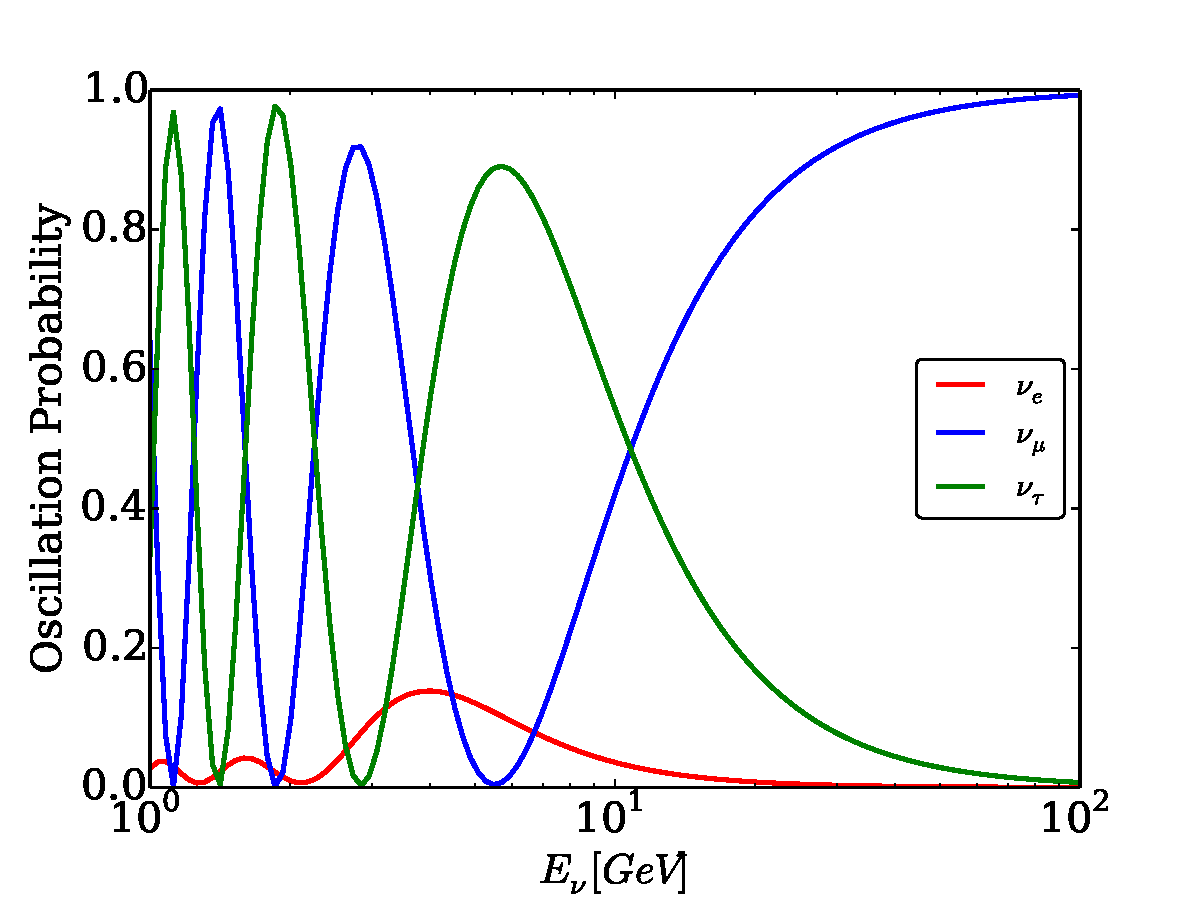
\includegraphics[width=0.8\textwidth]{../fig/earth_oscillation.pdf}
\caption{Single mode neutrino oscillation probability in a constant density matter environment.}
\end{center}
\end{figure}

In the above example we could had rather fix the energy and reset the {\ttf Track} in order to explore the probability as a function of baseline. 

\subsubsection{Example 3}

We can also use the custom environments provided, such as {\ttf ConstantDensity} and {\ttf VariableDensity}. For example in case we want to consider $\rho = 13 {\rm gr}/{\rm cm}^3$ and $y_e = 0.5$ we can use the code snipped in Listing \ref{ex:sin3}, which result is shown in Fig. \ref{fig:nu_mu_nue_single_energy},

\begin{lstlisting}[frame=leftline, numbers = left,breaklines=true, label = ex:sin3]
nuSQUIDS nus(3,"neutrino");
double phi = acos(-1.0);
std::vector<double> ini_state{0,1,0};
nus.Set_Body(std::make_shared<ConstantDensity>(13.0,0.5));
nus.Set_Track(std::make_shared<ConstantDensity::Track>(0.0,1000.0*nus.units.km));
for( double enu : energy_range ){
	nus.Set_E(enu);
	nus.Set_initial_state(ini_state,"flavor");
	nus.EvolveState();
	std::cout << nus.EvalFlavor(0) << std::endl;
}
\end{lstlisting}

\begin{figure}[h]
\begin{center}
\label{fig:nu_mu_nue_single_energy}
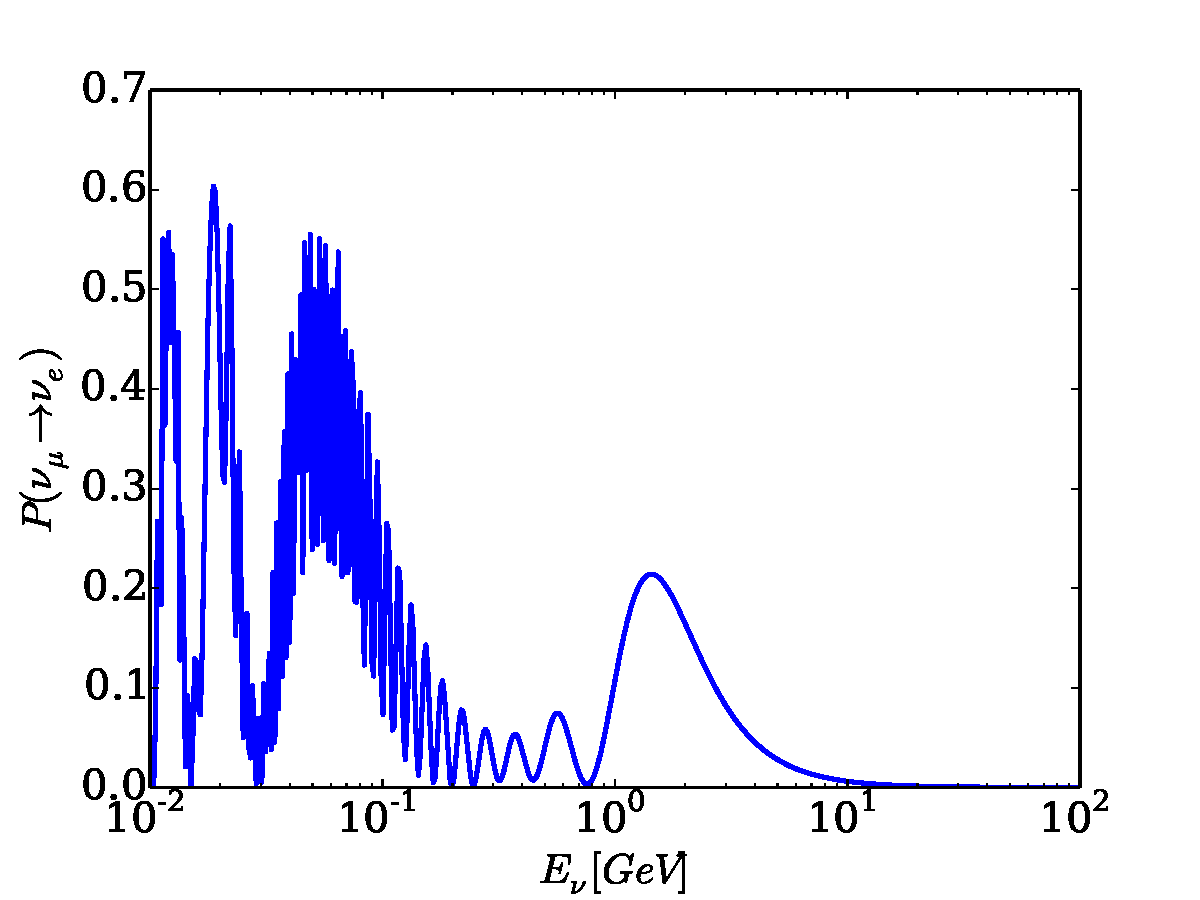
\includegraphics[width=0.8\textwidth]{../fig/nu_mu_nue_single_energy.pdf}
\caption{Single mode neutrino oscillation probability in a constant density matter environment.}
\end{center}
\end{figure}

\subsection{{\it Multiple} energy mode}

As explained in the text the {\it multiple} energy mode can consider a {\it set} of neutrino energies. The simplest thing that can be done is to 

\subsubsection{Example 1}

In this mode we can actually input a neutrino flux and propagate it in its environment. For example we could propagate $\phi(E) = \phi_0 E^{-1} \Pi_\mu$, i.e. power law pure $\nu_\mu$ flux, through the Earth. In Listing \ref{ex:mul1} we shall consider the this case and further demonstrate the how to consider more neutrino flavors. The results of the following code are shown in Figure \ref{fig:sterile_osc}.

\begin{lstlisting}[frame=leftline, numbers = left,breaklines=true, label = ex:mul1]
nuSQUIDS nus(1.,1.e2,200,4,"neutrino",true,false);

double phi = acos(-1.);
std::shared_ptr<EarthAtm> earth_atm = std::make_shared<EarthAtm>();
std::shared_ptr<EarthAtm::Track> track_atm = std::make_shared<EarthAtm::Track>(phi);

// set sterile parameters while leaving the rest at default
nus.Set("dm41sq", 3.0);
nus.Set("th24", 0.7);

nus.Set("rel_error", 1.0e-9);
nus.Set("abs_error", 1.0e-9);

// construct the initial state
vector<double> E_range = nus.GetERange();
array2D inistate(E_range.size());
double N0 = 1.0e18;
for ( int i = 0 ; i < inistate.size(); i++){
      inistate[i].resize(3);
      for ( int k = 0; k < 3; k ++){
        // initialze muon state
        inistate[i][k] = (k == 1) ? N0*pow(E_range[i],-2) : 0.0;
      }
}
// set the initial state
nus.Set_initial_state(inistate,"flavor");

nus.EvolveState();
// save the result
nus.WriteStateHDF5("./mulene_example1.hdf5");
\end{lstlisting}

\begin{figure}[h]
\begin{center}
\label{fig:sterile_osc}
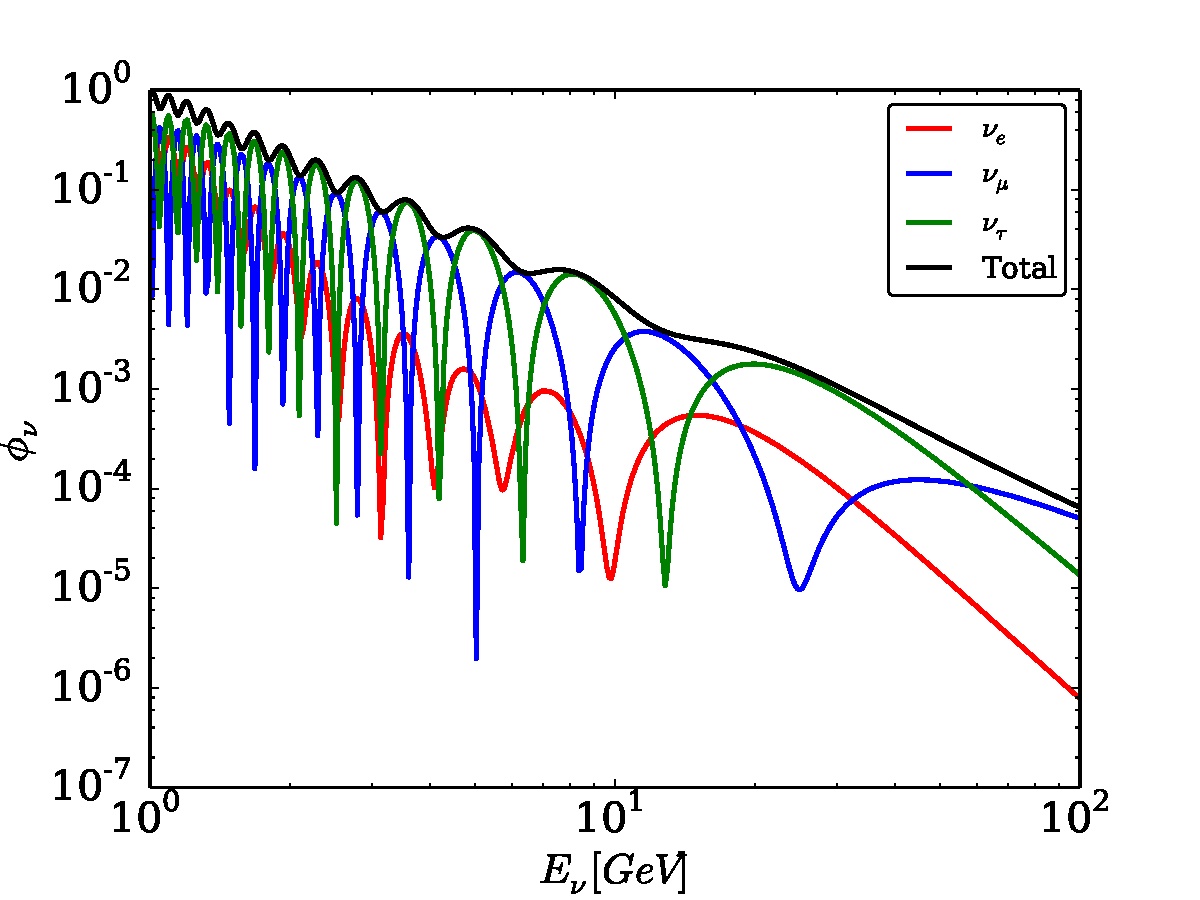
\includegraphics[width=0.8\textwidth]{../fig/sterile_osc_demo.pdf}
\caption{Single mode neutrino oscillation probability in a constant density matter environment.}
\end{center}
\end{figure}

\subsubsection{Example 2}

We can further consider the the propagation of $\phi(E) = \phi_0 E^{-1} ( \Pi_\mu + \Pi_\tau )$, again through the Earth, but considering $\tau$ regeneration. 

\begin{lstlisting}[frame=leftline, numbers = left,breaklines=true]

\end{lstlisting}

\section{Conclusions \& Acknowledgements} 
\label{sec:conclu} 

\bibliographystyle{elsarticle-harv}
\bibliography{nusquids}

\end{document}



